%!TEX root=../GaugeCNNTheory.tex


\subsection{Gauges, gauge transformations and \textit{G}-structures}
\label{sec:21_main}



\subsubsection{Tangent spaces and reference frames}
\label{sec:gauges_gauge_trafos}


A $d$-dimensional (smooth) manifold $M$ has a tangent space $\TpM\cong\R^d$ attached to each point $p\in M.$
The tangent spaces are $d$-dimensional vector spaces, however, in contrast to $\R^d$ they do in general not come with any preferred choice of reference frame.
A tangent vector $v\in \TpM$ is a \emph{coordinate free} object and is thus not immediately represented numerically by a coordinate tuple $(v_1,\dots,v_d)\in\R^d$.
More abstractly stated, each tangent space $\TpM$ is isomorphic~to~$\R^d$ but in general no canonical isomorphism between them is given.
Both spaces are therefore structurally equivalent but are not identified with each other in any preferred way.


A \emph{gauge} (local trivialization of the tangent bundle) on $U^A\subseteq M$ is defined as a smoothly position dependent collection of invertible linear maps
\begin{align}\label{eq:gauge_definition}
    \psi_p^A:\TpM\to\R^d \,,\ \ p\in U^A \,,
\end{align}
specifying the missing vector space isomorphisms between $\TpM$ and $\R^d$.
As visualized in Fig.~\ref{fig:gauge_trafos}, they coordinatize the tangent spaces by assigning a \emph{coefficient vector}
\begin{align}
    v^A\ :=\ \psi_p^A(v) \ \in\R^d
\end{align}
to each coordinate free tangent vector $v\in \TpM$.
An inversion of this relation yields
\begin{align}
    v\ =\ \left(\psi_p^A\right)^{-1}\! (v^A)
     \ =\ \left(\psi_p^A\right)^{-1}\!\! \left(\sum\nolimits_i v_i^A \epsilon_i\right)
     \ =\ \sum\nolimits_i v_i^A\, \left(\psi_p^A\right)^{-1}\!(\epsilon_i)
     \ =:\ \sum\nolimits_i v_i^A\, e_i^A \,,
\end{align}
where we denoted by $\{\epsilon_1,\dots,\epsilon_d\}$ the standard basis of $\R^d$ and made use of the linearity of the gauge to pull out the summation.
This shows that the gauge can be thought of as endowing each tangent space $\TpM$ with a \emph{reference frame}
\begin{align}\label{eq:framefield_gauge_equivalence}
    \left[e^A_{1}, \,\dots,\, e^A_{d}\right]
    \ :=\ \Big[(\psi_p^A)^{-1}(\epsilon_1), \:\dots\,,\; (\psi_p^A)^{-1}(\epsilon_d)\Big] \,,
\end{align}
defined as that $d$-tuple of linearly independent tangent vectors which results when mapping the standard frame of $\R^d$ back through the inverse gauge map.
For brevity, we will in the following use the shorthand notation $\big[e_i^A \big]_{i=1}^d$ for frames $\big[e_1^A, \dots, e_d^A \big]$.
The coefficients $v^A$ are the coordinates of $v$ relative to this frame.
The collection of frames induced by the $\psi_p^A$ on $U^A$ is called (smooth) \emph{frame field}; see Fig~\ref{fig:gauge_trafos_manifold} for a visualization.


\begin{figure}
    \centering
    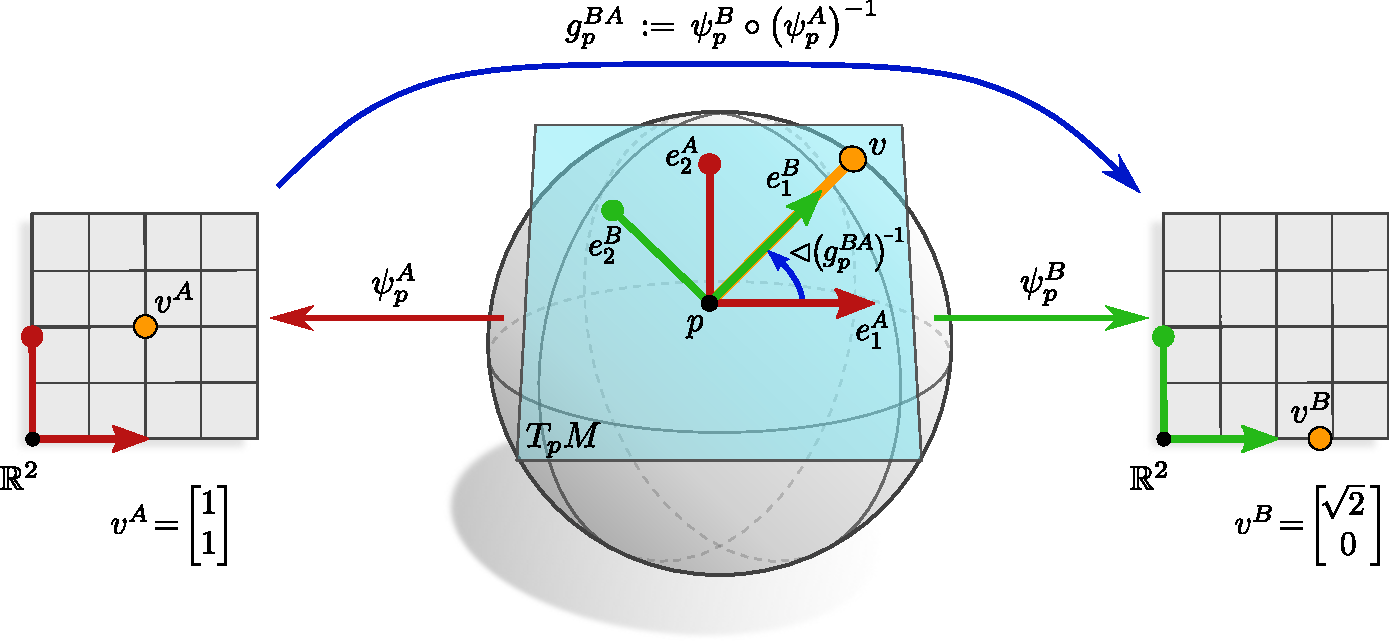
\includegraphics[width=\columnwidth]{figures/gauges_TpM.pdf}
    \caption{\small
        Identification of $\TpM\!\cong\!\R^2$ with $\R^2$ via different gauges.
        A (coordinate free) tangent vector $v\in \TpM$ (orange) can be represented numerically by a coordinate tuple $v^A=\psi_p^A(v)=\big(1,1\big)^\top$ relative to gauge $\psi_p^A$ (red) or, equivalently, by $v^B=\psi_p^B(v)=(\sqrt{2},0)^\top$ relative to gauge $\psi_p^B$ (green).
        A choice of gauge corresponds to a choice $[e_1^A,e_2^A]$ or $[e_1^B,e_2^B]$ of reference frame.
        On a general manifold no choice of gauge or coordinatization is preferred a~priori.
        Different gauges, and thus reference frames, are related by gauge transformations $g_p^{BA}:=\psi_p^B\circ(\psi_p^A)^{-1}$ (blue) which take values in the thus defined structure group $G$.
        This figure is a graphical interpretation of the commutative diagrams in Eq.~\eqref{eq:commutative_diagram_TpM} and Fig.~\ref{fig:trivialization_TM}.
        Note that gauges are immediately assigning coordinates to tangent spaces.
        Fig.~\ref{fig:affine_charts} in Section~\ref{sec:euclidean_geometry} shows a similar diagram for (affine) charts, which assign coordinates to the manifold, thereby \emph{inducing} gauges (``coordinate bases'').
        }
    \label{fig:gauge_trafos}
\end{figure}


Gauges $\psi^X$ coordinatize tangent spaces only on local neighborhoods $U^X\subseteq M$, and can due to topological obstructions in general not be extended to the whole manifold without violating the smoothness assumption.
One therefore considers an \emph{atlas}
\begin{align}
    \mathscr{A} \,=\, \big\{\! \big(U^X, \psi^X\big) \!\big\}_{X\in \mathfrak{X}} \,,
\end{align}
consisting of smooth gauges on a set of neighborhoods $U^X$ covering the manifold, that is, satisfying $\bigcup_{X\in \mathfrak{X}} U^X = M$, where $\mathfrak{X}$ is an index set.%
\footnote{
    An atlas of gauges is very similar to usual atlases of charts of a manifold (Appendix~\ref{apx:coordinate_bases}).
    The difference is that the here considered atlases directly assign coordinates to the tangent bundle $\TM$ instead of to the manifold $M$.
}
On the overlaps $U^A\cap U^B\neq\varnothing$ of neighborhoods, different gauges $\psi_p^A$ and $\psi_p^B$ are stitched together by smooth \emph{transition functions}%
\begin{align}\label{eq:transition_fct_local_def_21}
    g^{BA}\!:\, U^A\cap U^B\to\GL{d},\quad p \mapsto g_p^{BA} := \psi_p^B \circ \left(\psi_p^A\right)^{-1}.
\end{align}
Here we assume the codomain (for now) to be given by the \emph{general linear group} $\GL{d}$, consisting of all invertible matrices in $ \R^{d\times d}$, which explain the relation between any pair of vector space isomorphisms (gauges) or reference frames.
The action of such a transition function on a given gauge defines a \emph{gauge transformation}
\begin{align}\label{eq:gauge_trafo_local_def_21}
    \psi_p^B\ =\ g_p^{BA} \!\cdot \psi_p^A.
\end{align}
In terms of a commutative diagram, the relation between different gauges is visualized as:%
\footnote{
    \mbox{
        \emph{Diagrams} give a visual overview of functions and the spaces between which they map.
        For instance, the diagram
    }
    \begin{minipage}{.2\textwidth}
    ${
    \mkern30mu
    \begin{tikzcd}[column sep=30pt, row sep=8pt, ampersand replacement=\&]
        X
            \arrow[r, pos=.55, "f" description]
            \arrow[rd, "h\!"']
        \& Y
            \arrow[d, "\;g"]
        \\
        \& Z
    \end{tikzcd}}$
    \end{minipage}
    \hfill
    \begin{minipage}{.8\textwidth}
    implies that there are functions $f:X\to Y$, \ $g:Y\to Z$ and $h:X\to Z$.
    If the compositions of functions along \emph{all} paths with the same start and endpoint agree, the diagram is said to be \emph{commutative}.
    Our example diagram is commutative if (and only if) \ $h = g\circ f$ holds.
    \end{minipage}
}
\vspace*{-1ex}
\begin{equation}\label{eq:commutative_diagram_TpM}
\begin{tikzcd}[column sep=50pt, row sep=5pt, font=\normalsize]
    \R^d
        \arrow[rr, rounded corners, to path={ 
                -- ([yshift=4.5ex]\tikztostart.north) 
                --node[above, pos=.5]{\small$g_p^{BA} \mkern2mu\cdot$} ([yshift=4.5ex]\tikztotarget.north) 
                -- (\tikztotarget.north)
                }]
    & \TpM
        \arrow[l, "\psi_p^A"']
        \arrow[r, "\psi_p^B"]
    & \R^d
        \arrow[ll, rounded corners, to path={ 
                -- ([yshift=-4.5ex]\tikztostart.south) 
                --node[below, pos=.5]{\small$g_p^{AB} \mkern2mu\cdot \,=\, \big( g_p^{BA} \big)^{-1} \mkern2mu\cdot$} ([yshift=-4.5ex]\tikztotarget.south) 
                -- (\tikztotarget.south)
                }]
\end{tikzcd}
\vspace*{-1ex}%
\end{equation}
Compare this diagram to its graphical interpretation in Fig~\ref{fig:gauge_trafos}.


A gauge transformation alters the coordinatization of the tangent spaces such that the same coordinate free tangent vector $v$ is represented by a different component vector
\begin{align}\label{eq:components_leftaction}
  v^B\ =\ g_p^{BA}v^A \,.
\end{align}
Since a gauge corresponds to a choice of frame field, a gauge transformation corresponds to a transformation between frame fields.
Specifically, a frame $\big[e_i^A\big]_{i=1}^d = \big[e_1^A,\dots,e_d^A\big]$ at $p\in M$ transforms to another frame
\begin{alignat}{3}\label{eq:frame_rightaction}
    \qquad
    \left[e_{i}^B\right]_{i=1}^d\ \notag
    :=&\ \left[ \left(\psi_p^B\right)^{-1} (\epsilon_i) \right]_{i=1}^d
        \qquad\quad && \big( \text{\small gauge induced frame, Eq.~\eqref{eq:framefield_gauge_equivalence} } \big) \notag\\
    =&\ \left[ \left(g_p^{BA} \cdot \psi_p^A\right)^{-1} \left(\epsilon_i\right) \right]_{i=1}^d
        \qquad\quad && \big( \text{\small gauge trafo, Eq.~\eqref{eq:gauge_trafo_local_def_21}} \big) \notag\\
    =&\ \left[ \left(\psi_p^A\right)^{-1} \left(\left(g_p^{BA}\right)^{-1} \epsilon_i\right) \right]_{i=1}^d
        \qquad\quad && \big( \text{\small expanded inverse} \big) \notag\\
    =&\ \left[ \left(\psi_p^A\right)^{-1} \left(\sum\nolimits_j \epsilon_j \epsilon_j^\top \left(g_p^{BA}\right)^{-1} \epsilon_i\right) \right]_{i=1}^d
        \qquad\quad && \big( \text{\small inserted identity}\ {\textstyle\mathds{1}=\sum_j\epsilon_j\epsilon_j^\top}\ \big) \notag\\
    =&\ \left[ \left(\psi_p^A\right)^{-1} \left(\sum\nolimits_j \epsilon_j \left(\!\left(g_p^{BA}\right)^{-1}\right)_{ji} \right) \right]_{i=1}^d
        \qquad\quad && \big( \text{\small identified matrix elements of $\big(g_p^{BA}\big)^{-1}$} \big) \notag\\
    =&\ \left[ \sum\nolimits_j \left(\psi_p^A\right)^{-1}\! (\epsilon_j)\ \left(\!\left(g_p^{BA}\right)^{-1}\right)_{ji} \right]_{i=1}^d
        \qquad\quad && \big( \text{\small linearity of $\psi_p^A$} \big) \notag\\
    =&\ \left[ \sum\nolimits_j e_{j}^A \left(\!\left(g_p^{BA}\right)^{-1}\right)_{ji} \right]_{i=1}^d
        \qquad\quad && \big( \text{\small gauge induced frame, Eq.~\eqref{eq:framefield_gauge_equivalence} } \big) \notag\\
    =&\mkern-6mu: \left[ e_{i}^A \right]_{i=1}^d \lhd \left(g_p^{BA}\right)^{-1}
        \qquad\qquad &&
\end{alignat}
via the thus defined \emph{right action}
\begin{align}\label{eq:right_action_mapsto}
    \lhd:\ \pig( [e_i]_{i=1}^d,\ g \pig)\ \mapsto\ [e_i]_{i=1}^d \lhd g\, :=\,  \Big[ \sum\nolimits_j e_j\, g_{ji} \Big]_{i=1}^d
\end{align}
of group elements on frames.
Note that the inverse in this action in Eq.~\eqref{eq:frame_rightaction} is due to the definition of Eq.~\eqref{eq:gauge_trafo_local_def_21} without inverse.%
\footnote{
    Other conventions might flip the choice of inverses in
    $\psi^B = g^{BA}\psi^A$ and $[e_i^B]_{i=1}^d = [e_i^A]_{i=1}^d\lhd \big(g^{BA}\big)^{-1}\!$.
    An inverse in either of the two equations is necessary to make the left action $\cdot$ on gauges and right action $\lhd$ on frames compatible.
}
One usually refers to the transformation behavior of reference frames as \emph{covariant} transformation while the transformation of gauges and vector coefficients is denoted as \emph{contravariant} transformation; see Appendix~\ref{apx:coordinate_bases}.

\begin{SCfigure}
    \centering
    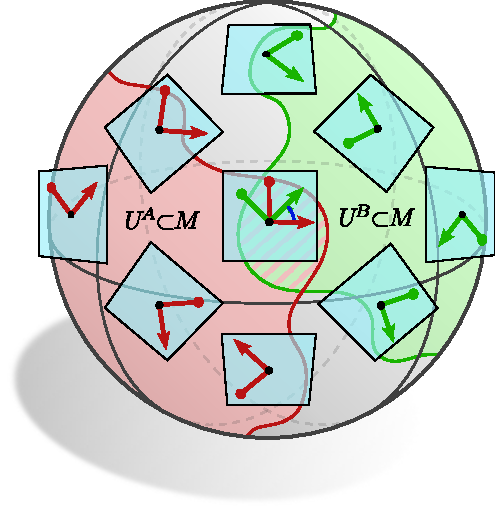
\includegraphics[width=.45\columnwidth]{figures/sphere_framefield.pdf}
    \captionsetup{width=.9\textwidth}
    \hspace{1ex}
    \caption{\small
        Each point $p$ of a Riemannian manifold $M$ has a tangent space $\TpM$ attached.
        A smooth gauge $\psi^A$ on a suitably chosen subset $U^A \subseteq M$ (red) coordinatizes all tangent spaces $\TpM$ for $p$ in $U^A$ as shown in Fig.~\ref{fig:gauge_trafos}.
        It is equivalent to a choice of \emph{smooth frame field} on $U^A$.
        Since it is in general not possible to extend a gauge globally over the whole manifold, it is necessary to consider a \mbox{$G$-\emph{atlas}}, consisting of gauges which cover $M$.
        Different coordinatizations $\psi^A$ on $U^A$ (red) and $\psi^B$ on $U^B$ (green) are patched together via gauge transformations (or transition maps) ${g^{BA}: U^A \cap U^B \to G}$ which are defined on the overlap ${U^A\cap U^B}$ (striped) and take values in the structure group $G \leq \GL{d}$.
        \\\protect\rule{0ex}{7.5ex}
        }
    \label{fig:gauge_trafos_manifold}
\end{SCfigure}


Since the transformation behavior of the coefficients in Eq.~\eqref{eq:components_leftaction} and the basis in Eq.~\eqref{eq:frame_rightaction} are inverse to each other they compensate, that is, they leave the tangent vector $v = \sum_i v_i^A e_{i}^A = \sum_i v_i^B e_{i}^B$ invariant:
\begin{align}\label{eq:vector_in_different_bases}
    v\ =\ \sum\nolimits_i v_i^B e_{i}^B
    \ &=\ \sum\nolimits_i v_i^B \sum\nolimits_j e_{j}^A \left(\left(g_p^{BA}\right)^{-1}\right)_{ji} \notag\\
    \ &=\ \sum\nolimits_j \left(\sum\nolimits_i \left(\left(g_p^{BA}\right)^{-1}\right)_{ji} v_i^B\right) e_{j}^A \notag\\
    \ &=\ \sum\nolimits_j v_j^A e_{j}^A \,.
\end{align}
This construction ensures that any calculation is ultimately independent of the chosen gauge, which is usually denoted as \emph{coordinate independence}.
In general, any coordinate representation of a coordinate free object or function is for consistency reasons required to be coordinate independent.


For completeness we want to mention that the here presented formalism defines general bases of the tangent spaces, sometimes referred to as \emph{non-coordinate bases} (non-holonomic bases), in terms of local gauges.
A~very popular but less general alternative are \emph{coordinate bases} (holonomic bases)
\begin{align}
    \bigg[\frac{\partial}{\partial x^A_1} \bigg|_p ,\,\dots\,,\ \frac{\partial}{\partial x^A_d} \bigg|_p \bigg] \,,
\end{align}
which are induced by \emph{coordinate charts}
\begin{align}\label{eq:chart_21}
    x^A: U^A \to V^A \subseteq \R^d
\end{align}
of the manifold \cite{nakahara2003geometry}.
The corresponding gauges are given by the the \emph{chart differentials}, that is,
\begin{align}
    \psi_p^A \,=\, \hat{d}x^A_p \,=\, \big( \hat{d}x^A_{p,1} \,,\dots,\, \hat{d}x^A_{p,d} \big)^\top\ :\ \TpM \to \R^d \,.
\end{align}
Gauge transformations coincide in this setting with the \emph{Jacobians}
\begin{align}
    g_p^{BA} \,=\, \frac{\partial x^B}{\partial x^A} \bigg|_{x^A(p)} \,\in\, \GL{d}
\end{align}
of chart transition maps.
An exemplary chart and its induced coordinate bases are visualized in Fig.~\ref{fig:sphere_chart}.
Appendix~\ref{apx:coordinate_bases} discusses the relationship between both formalisms in detail; an overview is given in Table~\ref{tab:coord_charts_gauge_trafos}.


\begin{figure}
    \centering
    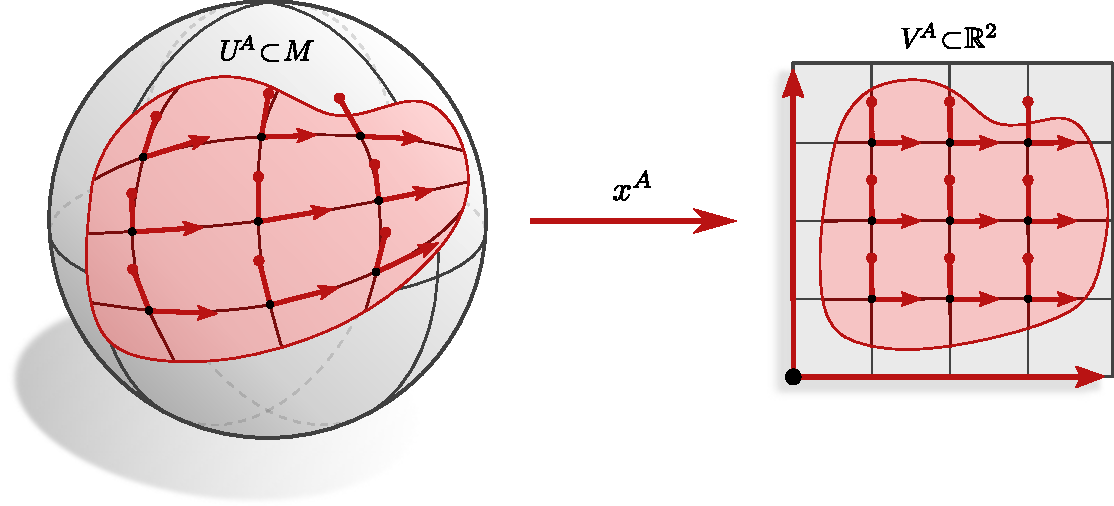
\includegraphics[width=.86\textwidth]{figures/sphere_chart.pdf}
    \hspace*{4ex}
    \caption{\small
        A \emph{chart} $x^A: U^A \to V^A$ assigns coordinates $V^A \subseteq \R^d$ to regions $U^A \subseteq M$ of the manifold.
        It induces \emph{coordinate bases}
        $\big[\frac{\partial}{\partial x^A_1} \big|_p ,\,\dots\,,\ \frac{\partial}{\partial x^A_d} \big|_p \big]$
        and corresponding gauges $\psi_p^A = \hat{d}x_p^A$ of the tangent spaces $\TpM$ over~$U^A$.
        We will mostly not work with charts but rather refer to points $p\in M$ in a \emph{coordinate free} manner.
        Gauges (frames) are then directly assigned to the tangent spaces instead of being induced.
    }
    \label{fig:sphere_chart}
\end{figure}


In the remainder of this paper we will mainly work in the gauge formalism, which assigns reference frames immediately to the tangent spaces instead of inducing them from charts.
Exceptions are
the M\"obius convolutions in Section~\ref{sec:mobius_conv},
Euclidean CNNs in Section~\ref{sec:instantiations_euclidean},
log-polar coordinates in Section~\ref{sec:polar_Euc2_logpolar}
and icosahedral CNNs in Section~\ref{sec:spherical_CNNs_icosahedral}.
In all of these cases the manifolds are \emph{locally flat} and the charts are \emph{isometric}, such that they induce \emph{orthonormal frames}.
$\GM$-convolutions on $U^A$ can then be computed in an efficient manner by running Euclidean convolutions with $G$-steerable kernels on the charts' codomains~$V^A$.











\subsubsection{Coordinate independent functions on tangent spaces}
\label{sec:gauges_TpM_functions}

Just as the vectors $v\in \TpM$, \emph{functions} on the tangent spaces are coordinate free, that is, they are defined without referring to any reference frame.
A chosen gauge allows to represent such coordinate free mappings by functions which operate on coefficient vectors in $\R^d$.
Similar to the coefficient vectors, coordinatizations of functions need to transform in a specific way under gauge transformations in order to be consistently defined, i.e. to respect coordinate independence.
We will later apply the here presented concept of expressing coordinate free mappings in terms of local coordinates to define $\GM$-coordinate independent convolutions.

\begin{figure}
    \centering
    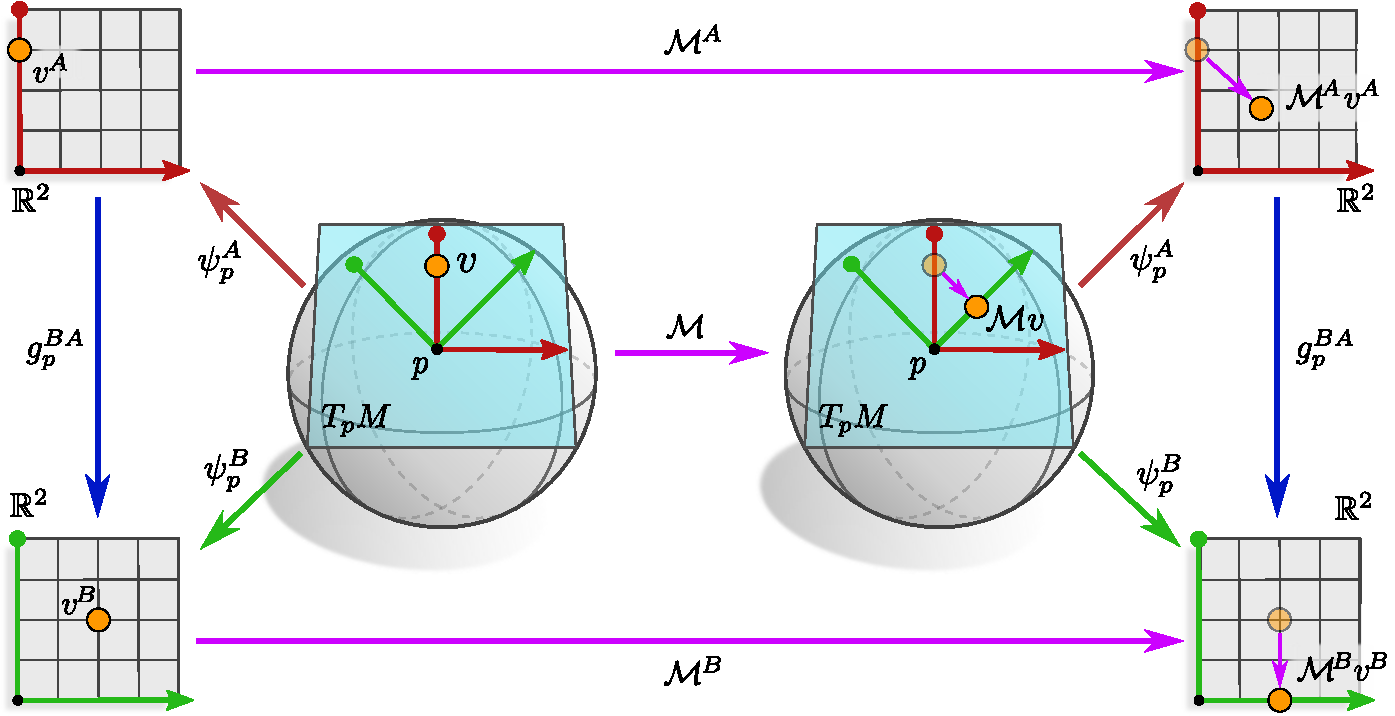
\includegraphics[width=\columnwidth]{figures/gauges_TpM_functions.pdf}
    \vspace*{.5ex}
    \caption{\small
            Graphical interpretation of the commutative diagram in Eq.~\eqref{eq:linear_map_TpM_diagram}.
            A coordinate free map $\mathcal{M}: \TpM \to \TpM$ can be equivalently represented by functions $\MAA\!: \R^d \to \R^d$ or $\MBB\!: \R^d \to \R^d$ \mbox{relative to different gauges $\psi_p^A$ or~$\psi_p^B$,} respectively.
            These coordinatizations of $\mathcal{M}$ are defined by a pre- and postcomposition with gauges in the domain and codomain, for instance, following the arrows, $\MAA := \psi_p^A \circ \mathcal{M} \circ \big(\psi_p^A\big)^{-1}$.
            As a consequence, gauge transformations $\MBB = g_p^{BA} \MAA \big(g_p^{BA}\big)^{-1}$ between coordinatizations are given by a pre- and postcomposition with transition maps~$g_p^{BA}$ in the domain and codomain.
            \emph{All} quantities and mappings in this work will either be coordinate free (like $\mathcal{M}$) or will be expressed in a coordinate independent way in different gauges (like $\MAA$ and $\MBB$).
            We will therefore need to define (or derive) transformation laws for any quantity and function.
        }
    \label{fig:gauge_trafos_functions}
\end{figure}

As a simple example for a coordinate free operation, let us consider the case of a \emph{linear map}
\begin{align}
    \mathcal{M}:\TpM\to \TpM \,.
\end{align}
Let $v_\text{in}\in \TpM$ be a tangent vector which is by $\mathcal{M}$ being mapped to $v_\text{out} = \mathcal{M} v_\text{in} \in \TpM$.
Linear maps are in numerical implementations usually modeled by \emph{coefficient matrices} which map between \emph{coefficient vectors} relative to some choice of reference frame.
To make this precise, assume some gauge $\psi_p^A$ to be given such that the coordinate free vectors $v_\textup{in}$ and $v_\textup{out}$ in $\TpM$ are represented by coefficient vectors $v_\text{in}^A=\psi_p^A(v_\text{in})$ and $v_\text{out}^A=\psi_p^A(v_\text{out})$ in~$\R^d$.
The linear map $\mathcal{M}$ is in this gauge represented by the matrix%
\begin{align}\label{eq:matrix_trivialization}
    \MAA\ :=\ \psi_p^A \circ \mathcal{M} \circ \big(\psi_p^A\big)^{-1} \ \ \in\ \R^{d\times d}
\end{align}
whose definition is visualized by the commutative diagram below:
\begin{equation}\label{eq:bundle_morphism_onexone}
\begin{tikzcd}[row sep=4.em, column sep=4.em]
    \R^d
            \arrow[rrr, pos=.5, rounded corners, to path={ 
                -- ([yshift=-3.5ex]\tikztostart.south) 
                --node[below]{\small$
                    \MAA
                    $} ([yshift=-3.5ex]\tikztotarget.south) 
                -- (\tikztotarget.south)
                    }]
    & \TpM  \arrow[r, "\mathcal{M}"]
            \arrow[l, "\psi_p^A"']
    & \TpM  \arrow[r, "\psi_p^A"]
    & \R^d
\end{tikzcd}
\end{equation}
The matrix is consistent with the coordinate free mapping since both imply each other:
\begin{align}
    \MAA v^A_\text{in}
    \ &=\ \pig[ \psi_p^A \circ \mathcal{M} \circ \big(\psi_p^A\big)^{-1} \pig] \circ \pig[ \psi_p^A(v_\text{in}) \pig] \notag \\
    \ &=\ \psi_p^A \big( \mathcal{M}\mkern2mu v_\text{in} \big) \notag \\
    \ &=\ \psi_p^A (v_\text{out}) \notag \\
    \ &=\ v_\text{out}^A
\end{align}
Of course one could have represented $\mathcal{M}$ relative to any other choice of gauge $\psi_p^B$.
We know from Eq.~\eqref{eq:components_leftaction} that coefficient vectors in different gauges are related by $v^B = g_p^{BA} v^A$.
Similarly, $\MBB$ relates to $\MAA$ by the gauge transformation
\begin{alignat}{2}\label{eq:matrix_gaugetrafo}
    \MBB
    \ &=&\ \ \psi_p^B \circ\, &\mathcal{M} \circ \big(\psi_p^B\big)^{-1} \notag \\
    \ &=&\ \ \psi_p^B \circ \big(\psi_p^A\big)^{-1} \circ\, &\MAA \circ \psi_p^A \circ \big(\psi_p^B\big)^{-1} \notag \\
    \ &=&\ \ g_p^{BA} &\MAA \big(g_p^{BA}\big)^{-1} \,,
\end{alignat}
which acts here both on the domain and codomain.%
\footnote{
    The transformation of the matrix coefficients via the left and right multiplication with $g^{BA}$ and $\big(g^{BA}\big)^{-1}$, respectively, identify the linear map as a tensor of type $(1,1)$.
}
This transformation law is again seen to be consistent by the mutual transformations canceling out:
\begin{align}
    \MBB v^B_\text{in}
    \ &=\ \pig[ g_p^{BA} \MAA \big(g_p^{BA}\big)^{-1} \pig]\, \pig[ g_p^{BA} v_\text{in}^A \pig] \notag \\
    \ &=\ g_p^{BA} \MAA v_\text{in}^A \notag \\
    \ &=\ g_p^{BA} v_\text{out}^A \notag \\
    \ &=\ v_\text{out}^B
\end{align}
The derived gauge transformations therefore assert that all coordinatized computations are ultimately coordinate independent.
The relations between the coordinate free mapping and its coordinatizations is summarized by the following commutative diagram
\begin{equation}\label{eq:linear_map_TpM_diagram}
\begin{tikzcd}[column sep=50pt, row sep=25pt, font=\normalsize]
    \R^d
        \arrow[dd, "g_p^{BA}\cdot\ "']
        \arrow[rrr, "\MAA"]
    & &[-2ex] &
    \R^d
        \arrow[dd, "\ g_p^{BA}\cdot"]
    \\
    &
    \TpM
        \arrow[ul, "\psi_p^A"]
        \arrow[dl, "\psi_p^B"']
        \arrow[r, "\mathcal{M}"]
    &
    \TpM
        \arrow[ur, "\psi_p^A"']
        \arrow[dr, "\psi_p^B"]
    \\
    \R^d
        \arrow[rrr, "\MBB"']
    & & &
    \R^d
\end{tikzcd}
\end{equation}
which is graphically interpreted in Fig.~\ref{fig:gauge_trafos_functions}.

In practice one can not instantiate the coordinate free linear map $\mathcal{M}$ numerically without referring to a choice of coordinatization.
However, its existence is implied if (and only if) its coordinatizations relate to each other as specified by Eq.~\eqref{eq:matrix_gaugetrafo}, which ensures that the correct transformation behavior of the input and output vector coefficients in Eq.~\eqref{eq:components_leftaction} is preserved.












\subsubsection{Structure groups, \textit{G}-structures and \textit{G}-atlases}
\label{sec:local_G-structure_G-atlas}

We will later on require neural networks to operate in a coordinate independent manner, that is, we demand their inference to be independent from arbitrary choices of reference frames.
This raises the question to which extent the choice of reference frames on a manifold is arbitrary.
In the previous Sections~\ref{sec:gauges_gauge_trafos} and~\ref{sec:gauges_TpM_functions} we allowed for any possible choice of gauge or reference frame, which were thus related by general $\GL{d}$-valued gauge transformations.
In many applications the manifold does, however, come with additional structure which allows to distinguish a \emph{preferred subset of reference frames} or gauges, whose transition functions take values in a \emph{reduced structure group} $G\leq\GL{d}$.
Such geometric structures -- or rather the subsets of preferred reference frames themselves, which encode equivalent information -- are denoted as \emph{$G$-structures}.


$G$-structures are best understood by considering some specific examples.
The following list gives such examples, classified by their structure group $G \leq \GL{d}$:
\begin{itemize}[leftmargin=9.4ex]
    \item[$\O{d}$:]
        Consider the \emph{metric} structure of a Riemannian manifold, which allows to measure distances and angels, and therefore to distinguish orthonormal frames, that is, those frames that satisfy $\eta(e_i,e_j) = \delta_{ij}$ for any $i,j=1,\dots,d$.
        Correspondingly, a Riemannian metric allows to talk about isometric gauges $\psi_p^A$, which identify the metric of $\R^d$ with that of~$\TpM$, i.e. which satisfy $\eta(v,w) = \langle \psi_p^A(v),\, \psi_p^A(w) \rangle_{\R^d}$ for any $v,w \in \TpM$.
        Since orthonormal frames and isometric gauges are defined up to rotations and reflections, any gauge transformation between them will take values in the orthogonal group~$\O{d}$, which is that subgroup of $\GL{d}$ that preserves angles and distances.
    \item[$\operatorname{GL}^+(d)$:]
        Similarly, an \emph{orientation} of the manifold distinguishes left-handed from right-handed frames and orientation preserving gauges from orientation reversing gauges.
        Gauge transformations between frames of a given handedness take values in $\operatorname{GL}^+(d)$, that is, that subgroup of $\GL{d}$ which preserves orientations.
    \item[$\SO{d}$:]
        Together, a given \emph{metric and orientation} specify orthonormal frames of a certain handedness.
        Gauge transformations between such frames are guaranteed to lie in the subgroup~$\SO{d}$ of $\GL{d}$.
    \item[$\{e\}$:]
        A \emph{globally smooth frame field} defines an $\{e\}$-structure on $M$.
        In this case there is only one single distinguished frame at each position, such that gauge transformations lie in the trivial group ${\{e\} \leq \GL{d}}$.
    \item[$\GL{d}$:]
        If no additional structure is imposed, \emph{any} reference frame of the tangent spaces is equally valid.
        Gauge transformations are in this case general invertible liner maps in $\GL{d}$ and the corresponding $G$-structure is just the frame bundle $\FM$.
\end{itemize}


\begin{samepage}
The common theme in those motivating examples is that they are all defined by
\begin{enumerate}
    \item a (spatially smoothly varying) subset of distinguished reference frames,
    \item a corresponding subset of preferred gauges and
    \item a subgroup $G \leq \GL{d}$ of gauge transformations which preserve the distinguished notion of\\ frames and gauges.
\end{enumerate}
\end{samepage}
Such smoothly varying subsets of reference frames are denoted as \emph{$G$-structures}~$\GM$ on~$M$
and the group~$G$ is denoted as (reduced) \emph{structure group}
-- see Section~\ref{sec:G_associated_bundles} for a more rigorous definition.%
\footnote{
    Formally, $\GM$ is defined as a principal $G$-subbundle of frame bundle $\FM$, which is a principal $\GL{d}$-bundle.
}
The process of specifying a $G$-structure is known as a \emph{reduction of the structure group} from $\GL{d}$ to~$G$.
An atlas ${\mathscr{A}^G = \big\{\! \big(U^X, \psi^X\big) \!\big\}_{X\in \mathfrak{X}}}$ is denoted as $G$\emph{-atlas} if all of its transition functions
\begin{align}\label{eq:transition_fct_local_def_21_G_atlas}
    g^{BA}\!:\, U^A\cap U^B\to G, \quad p \mapsto g_p^{BA} := \psi_p^B \circ \left(\psi_p^A\right)^{-1}
\end{align}
lie in a reduced structure group~$G \leq \GL{d}$ (cf. Eq.~\eqref{eq:transition_fct_local_def_21}).
The relation between reference frames and gauges in Eq.~\eqref{eq:framefield_gauge_equivalence} implies that any $G$-atlas encodes a corresponding $G$-structure.


Multiple choices of $G$-structures may exist for a given structure group~$G$.
To connect to the examples above:
different Riemannian metrics specify different subsets of reference frames as being orthonormal, that is, they correspond to different $\O{d}$-structures $\OM$.
A choice of metric is therefore equivalent to a choice of $\O{d}$-structure.
Similarly, different choices of orientations of an orientable manifold specify a different set of frames as being right-handed.
The two possible choices of orientations therefore correspond to two possible choices of $\operatorname{GL}^+(d)$-structures $\operatorname{GL}^+\mkern-5muM$.
$\SO{d}$-structures $\SOM$ may differ in both the choice of orientation and metric.
A further example are $\{e\}$-structure $\eM$.
They do not allow for (non-trivial) gauge transformations and therefore correspond to choices of smooth, global frame fields on $M$.
Table~\ref{tab:G_structures} gives more examples of structure groups~$G$ and the corresponding $G$-structures.


\begin{table}
    \centering
    \renewcommand\arraystretch{1.1}
    \small
    \begin{tabular}{cll}
       \toprule
       structure group $G\leq\GL{d}$ & $G$-structure $\GM$                      & equivalent structure on $M$       \\[.25ex]
       \midrule
       $\operatorname{GL}^+(d)$      & positively oriented frames               & orientation of $M$                \\
       $\operatorname{SL}(d)$        & unit volume frames                       & volume form                       \\
       $\operatorname{CO}(d)$        & conformal frames                         & ---                                \\
       $\operatorname{Sp}(d)$        & symplectic frames                        & ---                                \\
       $\operatorname{O}(d)$         & orthonormal frames                       & Riemannian metric                 \\
       $\operatorname{O}(d-n,\,n)$   & pseudo-orthonormal frames                & pseudo-Riemannian metric          \\
       $\operatorname{SO}(d)$        & positively oriented orthonormal frames   & Riemannian metric + orientation   \\
       $\{e\}$                       & parallelization (global frame field)     & ---                                \\[.25ex]
       \bottomrule
    \end{tabular}
    \vspace*{2ex}
    \caption{
        Examples of $G$-structures $\GM$ on $M$ and their corresponding, reduced structure groups~$G\leq\GL{d}$~\cite{kobayashi1972transformation}.
        A~$G$-structure is defined as a smoothly varying subset of reference frames (a principal $G$-subbundle of the frame bundle $\FM$), where the frames of any tangent space are mutually related by $G$-valued gauge transformations.
        While this is a quite abstract definition, it allows to view many geometric structures on~$M$ in a unified way.
        For instance, a Riemannian metric on~$M$ allows to distinguish orthonormal frames.
        Conversely, a specification of orthonormality uniquely implies a metric.
        A Riemannian metric and an orthonormal structure are thus equivalent to each other.
        Similarly, there is a one-to-one correspondence between volume forms and unit volume frames.
        Note that a choice of structure group $G$ does not uniquely specify a $G$-structure.
        For example, different Riemannian metrics could be chosen as $\O{d}$-structure, different volume forms as $\operatorname{SL}(d)$-structure or different global frame fields as $\{e\}$-structure.
        Coordinate independent CNNs are designed to respect a given $G$-structure -- which particular structure this is depends on the learning task.
    }
    \label{tab:G_structures}
\end{table}


A reduction of the structure group to $G$, i.e. the existence of a $G$-structure, might be obstructed by the topology of the manifold.
This implies that there is an \emph{``irreducible'' structure group} beyond which the ambiguity of reference frames can not be resolved without violating the smoothness (or even continuity) assumption of the $G$-structure.
For example, the M\"obius strip in is non-orientable, which means that it does not admit a globally consistent, smooth definition of frame handedness and thus $\{e\}$-structure (globally smooth frame field).
As~visualized in Fig.~\ref{fig:mobius_conv_gauges}, a $G$-atlas of gauges covering the M\"obius strip will unavoidably require a reflection in one of the transition maps, implying an irreducible structure group $G=\Flip$.
Coordinate independent CNNs on the M{\"o}bius strip is therefore required to be at least reflection equivariant.
Similarly, the structure group of the sphere can not be reduced further than ${G=\SO2}$.
Smooth spherical CNNs are thus necessarily based on locally rotation equivariant kernels.


Note that \emph{any} (differentiable) manifold comes with \emph{some} $G$-structure.
For instance, a raw differentiable manifold has a $\GL{d}$-structure (containing any possible frame), a Riemannian manifold an $\O{d}$-structure and $\R^d$ is canonically equipped with an $\{e\}$-structure, visualized in Fig.~\ref{fig:frame_field_automorphism_1}.
We will therefore without loss of generality refine the term ``coordinate independence'' to $\GM$-\emph{coordinate independence}, i.e. the independence w.r.t. choices of reference frames in the $G$-structure given on~$M$.
Throughout this work we will assume that gauges are part of some $G$-atlas
\begin{align}\label{eq:G_atlas_dfn}
    \mathscr{A}^G \,=\, \big\{\! \big(U^X, \psi^X\big) \!\big\}_{X\in \mathfrak{X}}
    \quad\ \textup{such that} \quad
    g_p^{BA} \in G
    \quad \textup{for any}\ \ \ \psi_p^A, \psi_p^B \in \mathscr{A}^G,\ \ p\in U^A\cap U^B \,,
\end{align}
corresponding to the given $G$-structure.
Any quantity or function can be expressed relative to any gauge from this atlas%
\footnote{
    This is a non-trivial statement since not any quantity can be expressed relative to arbitrary $\GL{d}$-related reference frames.
    For instance, the feature fields, introduced in Section~\ref{sec:feature_fields}, will only admit $G$-valued gauge transformations and are therefore only defined relative to the preferred frames in~$\GM$.
    As an intuitive example, consider the feature vectors of a conventional (non-equivariant) CNN on $\R^d$, which are extracted relative to the canonical $\{e\}$-structure of $\R^d$ and do \emph{not} carry information about the kernel responses relative to other reference frames.
},
and the coordinatizations in different gauges relate uniquely by some $G$-valued gauge transformation.
Guaranteeing the coordinate independence of all constructions, they will always correspond to some coordinate-free counterparts, in terms of which we will formulate the global theory in Sections~\ref{sec:bundles_fields}, \ref{sec:gauge_CNNs_global} and~\ref{sec:isometry_intro}.
